\documentclass[preprint,amsmath,amssymb,aps, prb,showkeys]{revtex4-1}
\usepackage{graphicx}% Include figure files
\usepackage{color,soul}
\usepackage{tabularx}
\usepackage{fullpage,subcaption,float,psfrag,textcomp,gensymb,tikz,siunitx}
\usepackage{booktabs,multirow, dcolumn}% Align table columns on decimal point
\usepackage{xspace}
\usepackage[mathscr]{euscript}
\usepackage{amsmath}
\usepackage{float}

\usepackage[bookmarks=true,pdftoolbar=true]{hyperref}
\hypersetup{%
  pdftitle = {MAX Phases: Supplementary text},
  pdfkeywords = {pdf, hyperref, bookmarks},
  pdfauthor = {Anjana Talapatra}}
 \usepackage[all]{hypcap} 


\graphicspath{{supplementary_figures/}}

\begin{document}

\section{Supplementary Information}
\label{sec:app}

\subsection{Features: Correlation Matrix}

\begin{figure}[h!]
\centering
\includegraphics[width=0.99\columnwidth]{correlation_matrix}
\caption{Pearson correlation matrix for the features used in this work. Small (lighter) values correspond to feature pairs with little correlation between them.}
\label{fig:Pearson}
\end{figure}


A Pearson correlation matrix  \cite{pearson1895notes} was calculated for all the features and is shown in Fig.\ref{fig:Pearson}. A Pearson coefficient $\rho$, is a linear correlation measure between two features $f_1$ and $f_2$ and may be calculated as:
\begin{equation}
\rho_{f_1,f_2} = \frac{cov (f_1,f_2)}{\sigma_{f_1} \sigma_{f_2}},
\end{equation}
where $cov$ denotes the covariance, $\sigma_{f_1}$ is the standard deviation of $f_1$, and $\sigma_{f_2}$ is the standard deviation of $f_2$. The value of the coefficient lies in $[-1,1]$, with $1$ indicating perfect positive linear correlation and $-1$ indicating perfect negative linear correlation. The goal is to get the best results possible by using the minimum number of features. Ideally, the feature pairs should be uncorrelated, which will ensure that we are not needlessly increasing the dimensionality of the feature space without substantially improving the results. Highly correlated features can be redundant and are undesirable, since they will increase the dimensionality of the feature space without proportionally increasing the information available to optimize the objective function.


\subsection{Model Benchmarking}

\begin{figure}[h!]
    \centering
    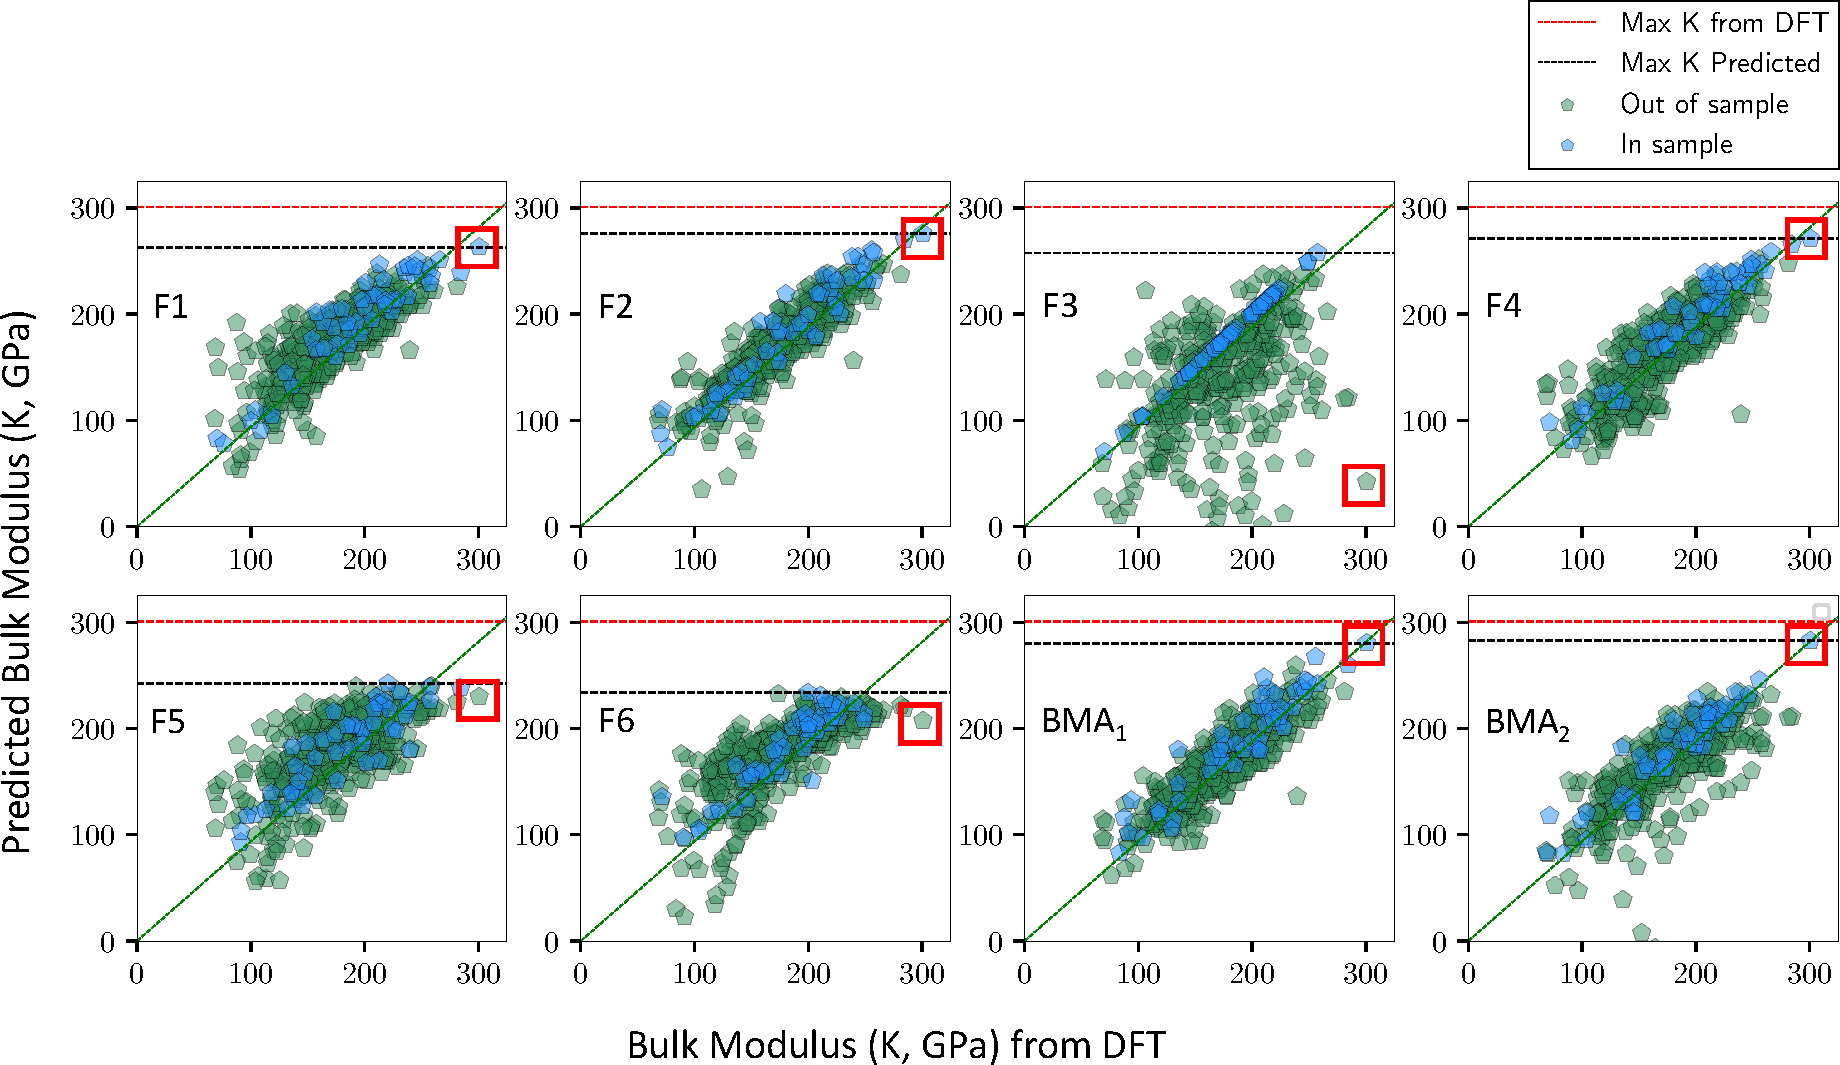
\includegraphics[scale=0.45]{error_estimation.pdf}
    \caption{In a single trial, after ten initial(N=10) and forty subsequent measurements, the GP model is fit to the n = 50  training points (in blue), and applied both to in-sample and out-of-sample data. Here, the red dashed line  corresponds to the largest DFT value seen so far, and the black dashed line  is the largest estimated value. Composition with the largest K value from DFT is highlighted (red square) to show the model error.}
    \label{fig:error_estimation}
\end{figure}


Figure \ref{fig:error_estimation} shows the results for one example of maximization of bulk modulus for all the feature sets and the BMA approach. The example started with 10 measured values, and after forty measurements, there are now 50 materials with known bulk modulus (K). These are then used to train the regressor;  and the predicted K and actual K (from DFT) are plotted for all of the materials (in green), including those in blue whose true K values are known (in blue). It can be seen that the model error is high for F$_3$, F$_5$ and F$_6$ and low for F$_1$, F$_2$, F$_4$, BMA$_1$ and BMA$_2$. This is akin to the results included in the manuscript. In figure \ref{fig:error_bar}, we visualize the bulk modulus estimated from GP model in all cases for the composition with the largest K value from DFT. Error bars indicate the variance of the GP model. It is seen that GP models based off both BMA$_1$ and BMA$_2$ get very close to the ground truth similar to F$_2$. Thus, inspite of poor performing models based off F$_3$, F$_5$ and F$_6$, the GP models based off the BMA approach perform as well as the best standalone model F$_2$

\begin{figure}[h!]
    \centering
    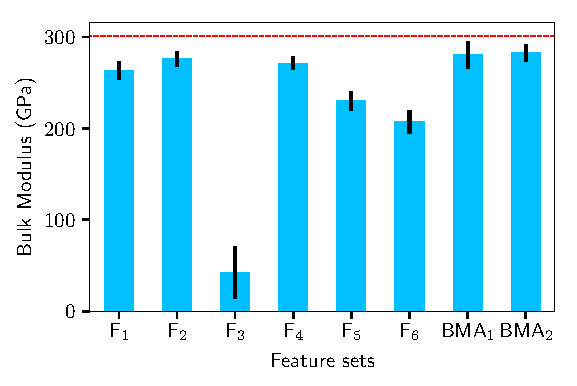
\includegraphics[scale=1]{error_bar_plot.pdf}
    \caption{Bar plots showing  estimated bulk modulus for the composition with the largest bulk modulus from DFT for all cases in a single trial, after ten initial(N=10) and forty subsequent measurements, the GP model is fit to the n = 50  training points, and applied both to in-sample and out-of-sample data. Error bars indicate the variance of the GP model. Red dashed line corresponds to target maximum bulk modulus from DFT. }
    \label{fig:error_bar}
\end{figure}

\newpage

\subsection{Additional Results}

\begin{figure}[htp]
        \parbox{.975\textwidth}{
            \begin{subfigure}{.475\linewidth}
                \includegraphics[width=\textwidth]{N_2_K_max_single_models}
                \caption{N=2}
                \label{fig:Max_bulk_N_2_single_models}
        \end{subfigure}
        	\begin{subfigure}{.475\linewidth}
                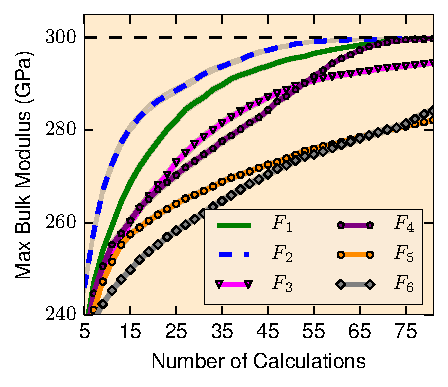
\includegraphics[width=\textwidth]{N_5_K_max_single_models}
                \caption{N=5}
                \label{fig:Max_bulk_N_5_single_models}
        \end{subfigure}
        	\begin{subfigure}{.475\linewidth}
                \includegraphics[width=\textwidth]{N_15_K_max_single_models}
                \caption{N=15}
                \label{fig:Max_bulk_N_15_single_models}
        \end{subfigure}
        	\begin{subfigure}{.475\linewidth}
                \includegraphics[width=\textwidth]{N_20_K_max_single_models}
                \caption{N=20}
                \label{fig:Max_bulk_N_20_single_models}
        \end{subfigure}
        }
        \caption{ Results for single objective optimization - maximization of bulk modulus. Average maximum bulk modulus discovered using all described feature sets for a) N=2, b) N=5, c) N=15, d) N=20.}
        \label{fig:Max_bulk_modulus_single}        
\end{figure} 

\begin{figure}[htp]
        \parbox{.975\textwidth}{
            \begin{subfigure}{.475\linewidth}
                \includegraphics[width=\textwidth]{K_max_N_2}
                \caption{N=2}
                \label{fig:Max_bulk_N_2_swarm}
        \end{subfigure}
        	\begin{subfigure}{.475\linewidth}
                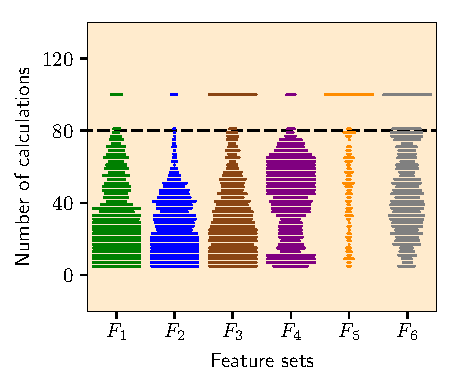
\includegraphics[width=\textwidth]{K_max_N_5}
                \caption{N=5}
                \label{fig:Max_bulk_N_5_swarm}
        \end{subfigure}
        	\begin{subfigure}{.475\linewidth}
                \includegraphics[width=\textwidth]{K_max_N_15}
                \caption{N=15}
                \label{fig:Max_bulk_N_15_swarm}
        \end{subfigure}
        	\begin{subfigure}{.475\linewidth}
                \includegraphics[width=\textwidth]{K_max_N_20}
                \caption{N=20}
                \label{fig:Max_bulk_N_20_swarm}
        \end{subfigure}
        }
        \caption{ Results for single objective optimization - maximization of bulk modulus. Swarm plots indicating the distribution of the number of calculations required for convergence using all described feature sets for a) N=2, b) N=5, c) N=15, d) N=20.}
        \label{fig:Max_bulk_modulus_swarm}        
\end{figure} 

\begin{figure}[htp]
        \parbox{.975\textwidth}{
            \begin{subfigure}{.475\linewidth}
                \includegraphics[width=\textwidth]{N_2_K_max_BMA}
                \caption{N=2}
                \label{fig:Max_bulk_N_2_BMA}
        \end{subfigure}
        	\begin{subfigure}{.475\linewidth}
                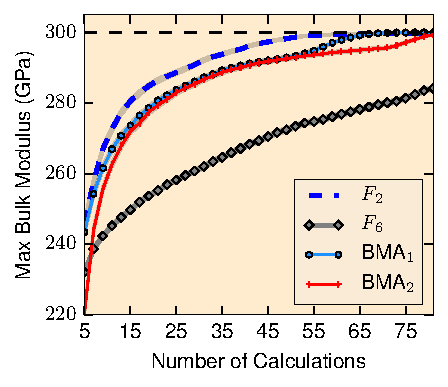
\includegraphics[width=\textwidth]{N_5_K_max_BMA}
                \caption{N=5}
                \label{fig:Max_bulk_N_5_BMA}
        \end{subfigure}
        	\begin{subfigure}{.475\linewidth}
                \includegraphics[width=\textwidth]{N_15_K_max_BMA}
                \caption{N=15}
                \label{fig:Max_bulk_N_15_BMA}
        \end{subfigure}
        	\begin{subfigure}{.475\linewidth}
                \includegraphics[width=\textwidth]{N_20_K_max_BMA}
                \caption{N=20}
                \label{fig:Max_bulk_N_20_BMA}
        \end{subfigure}
        }
        \caption{ Results for single objective optimization - maximization of bulk modulus. Average maximum bulk modulus discovered using the best feature set $F_2$, worst feature set $F_6$, BMA$_1$ and BMA$_2$ for a) N=2, b) N=5, c) N=15, d) N=20.}
        \label{fig:Max_bulk_modulus_single_BMA}       
\end{figure} 

\begin{figure}[htp]
        \parbox{.975\textwidth}{
            \begin{subfigure}{.475\linewidth}
                \includegraphics[width=\textwidth]{K_max_N_2_BMA_violinplot}
                \caption{N=2}
                \label{fig:Max_bulk_N_2_BMA_swarm}
        \end{subfigure}
        	\begin{subfigure}{.475\linewidth}
                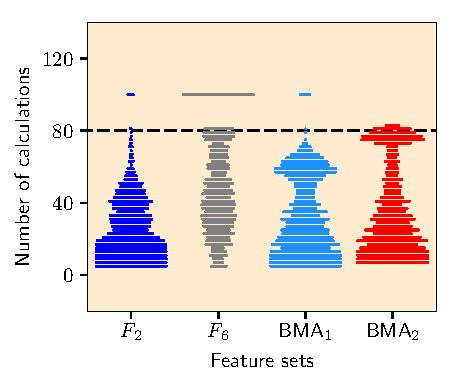
\includegraphics[width=\textwidth]{K_max_N_5_BMA_violinplot}
                \caption{N=5}
                \label{fig:Max_bulk_N_5_BMA_swarm}
        \end{subfigure}
        	\begin{subfigure}{.475\linewidth}
                \includegraphics[width=\textwidth]{K_max_N_15_BMA_violinplot}
                \caption{N=15}
                \label{fig:Max_bulk_N_15_BMA_swarm}
        \end{subfigure}
        	\begin{subfigure}{.475\linewidth}
                \includegraphics[width=\textwidth]{K_max_N_20_BMA_violinplot}
                \caption{N=20}
                \label{fig:Max_bulk_N_20_BMA_swarm}
        \end{subfigure}
        }
        \caption{ Results for single objective optimization - maximization of bulk modulus. Swarm plots indicating the distribution of the number of calculations required for convergence using best feature set $F_2$, worst feature set $F_6$, BMA$_1$ and BMA$_2$. a) N=2, b) N=5, c) N=15, d) N=20.}
        \label{fig:Max_bulk_modulus_BMA_swarm}
        
\end{figure} 

\begin{figure}[htp]
        \parbox{.975\textwidth}{
            \begin{subfigure}{.475\linewidth}
                \includegraphics[width=\textwidth]{N_2_K_max_BMA_first_order_coeff}
                \caption{N=2}
                \label{fig:K_max_fo_coeff_N_2_BMA}
        \end{subfigure}
            \begin{subfigure}{.475\linewidth}
                \includegraphics[width=\textwidth]{N_5_K_max_BMA_first_order_coeff}
                \caption{N=5}
                \label{fig:K_max_fo_coeff_N_5_BMA}
        \end{subfigure}
            \begin{subfigure}{.475\linewidth}
                \includegraphics[width=\textwidth]{N_15_K_max_BMA_first_order_coeff}
                \caption{N=15}
                \label{fig:K_max_fo_coeff_N_15_BMA}
        \end{subfigure}
            \begin{subfigure}{.475\linewidth}
                \includegraphics[width=\textwidth]{N_20_K_max_BMA_first_order_coeff}
                \caption{N=20}
                \label{fig:K_max_fo_coeff_N_20_BMA}
        \end{subfigure}
        }
        \caption{ Results for single objective optimization - maximization of bulk modulus. Average model probabilities for maximizing bulk modulus using BMA$_1$ for a) N=2, b) N=5, c) N=15, d) N=20.}
        \label{fig:K_max_fo_coeff_BMA}
       
\end{figure} 

\begin{figure}[htp]
        \parbox{.975\textwidth}{
            \begin{subfigure}{.475\linewidth}
                \includegraphics[width=\textwidth]{N_2_K_max_BMA_second_order_coeff}
                \caption{N=2}
                \label{fig:K_max_so_coeff_N_2_BMA}
        \end{subfigure}
            \begin{subfigure}{.475\linewidth}
                \includegraphics[width=\textwidth]{N_5_K_max_BMA_second_order_coeff}
                \caption{N=5}
                \label{fig:K_max_so_coeff_N_5_BMA}
        \end{subfigure}
            \begin{subfigure}{.475\linewidth}
                \includegraphics[width=\textwidth]{N_15_K_max_BMA_second_order_coeff}
                \caption{N=15}
                \label{fig:K_max_so_coeff_N_15_BMA}
        \end{subfigure}
            \begin{subfigure}{.475\linewidth}
                \includegraphics[width=\textwidth]{N_20_K_max_BMA_second_order_coeff}
                \caption{N=20}
                \label{fig:K_max_so_coeff_N_20_BMA}
        \end{subfigure}
        }
        \caption{ Results for single objective optimization - maximization of bulk modulus. Average model probabilities for maximizing bulk modulus using BMA$_2$ for a) N=2, b) N=5, c) N=15, d) N=20.}
        \label{fig:K_max_so_coeff_BMA}
    
\end{figure} 

\begin{figure}[htp]
        \parbox{.975\textwidth}{
            \begin{subfigure}{.475\linewidth}
                \includegraphics[width=\textwidth]{N_2_G_min_single_models}
                \caption{N=2}
                \label{fig:Min_G_N_2_single_models}
        \end{subfigure}
        	\begin{subfigure}{.475\linewidth}
                \includegraphics[width=\textwidth]{N_5_G_min_single_models}
                \caption{N=5}
                \label{fig:Min_G_N_5_single_models}
        \end{subfigure}
        	\begin{subfigure}{.475\linewidth}
                \includegraphics[width=\textwidth]{N_15_G_min_single_models}
                \caption{N=15}
                \label{fig:Min_G_N_15_single_models}
        \end{subfigure}
        	\begin{subfigure}{.475\linewidth}
                \includegraphics[width=\textwidth]{N_20_G_min_single_models}
                \caption{N=20}
                \label{fig:Min_G_N_20_single_models}
        \end{subfigure}
        }
        \caption{ Results for single objective optimization - minimization of shear modulus. Average minimum shear modulus discovered using all described feature sets for a) N=2, b) N=5, c) N=15, d) N=20.}
        \label{fig:min_shear_modulus_single_BMA}
         
\end{figure} 

\begin{figure}[htp]
        \parbox{.975\textwidth}{
            \begin{subfigure}{.475\linewidth}
                \includegraphics[width=\textwidth]{G_min_N_2}
                \caption{N=2}
                \label{fig:Min_G_N_2_swarm}
        \end{subfigure}
            \begin{subfigure}{.475\linewidth}
                \includegraphics[width=\textwidth]{G_min_N_5}
                \caption{N=5}
                \label{fig:Min_G_N_5_swarm}
        \end{subfigure}
            \begin{subfigure}{.475\linewidth}
                \includegraphics[width=\textwidth]{G_min_N_15}
                \caption{N=15}
                \label{fig:Min_G_N_15_swarm}
        \end{subfigure}
            \begin{subfigure}{.475\linewidth}
                \includegraphics[width=\textwidth]{G_min_N_20}
                \caption{N=20}
                \label{fig:Min_G_N_20_swarm}
        \end{subfigure}
        }
        \caption{ Results for single objective optimization - minimization of shear modulus. Swarm plots indicating the distribution of the number of calculations required for convergence using all described feature sets for a) N=2, b) N=5, c) N=15, d) N=20.}
        \label{fig:Min_G_modulus_swarm}
        
\end{figure}

\begin{figure}[htp]
        \parbox{.975\textwidth}{
            \begin{subfigure}{.475\linewidth}
                \includegraphics[width=\textwidth]{N_2_G_min_BMA}
                \caption{N=2}
                \label{fig:Min_G_N_2_BMA}
        \end{subfigure}
            \begin{subfigure}{.475\linewidth}
                \includegraphics[width=\textwidth]{N_5_G_min_BMA}
                \caption{N=5}
                \label{fig:Min_G_N_5_BMA}
        \end{subfigure}
            \begin{subfigure}{.475\linewidth}
                \includegraphics[width=\textwidth]{N_15_G_min_BMA}
                \caption{N=15}
                \label{fig:Min_G_N_15_BMA}
        \end{subfigure}
            \begin{subfigure}{.475\linewidth}
                \includegraphics[width=\textwidth]{N_20_G_min_BMA}
                \caption{N=20}
                \label{fig:Min_G_N_20_BMA}
        \end{subfigure}
        }
        \caption{ Results for single objective optimization - minimization of shear modulus. Average minimum shear modulus discovered using the best feature set $F_2$, worst feature set $F_6$, BMA$_1$ and BMA$_2$ for a) N=2, b) N=5, c) N=15, d) N=20.}
        \label{fig:Min_G_single_BMA}       
\end{figure} 

\begin{figure}[htp]
        \parbox{.975\textwidth}{
            \begin{subfigure}{.475\linewidth}
                \includegraphics[width=\textwidth]{G_min_N_2_BMA_violinplot}
                \caption{N=2}
                \label{fig:min_G_N_2_BMA_swarm}
        \end{subfigure}
            \begin{subfigure}{.475\linewidth}
                \includegraphics[width=\textwidth]{G_min_N_5_BMA_violinplot}
                \caption{N=5}
                \label{fig:min_G_N_5_BMA_swarm}
        \end{subfigure}
            \begin{subfigure}{.475\linewidth}
                \includegraphics[width=\textwidth]{G_min_N_15_BMA_violinplot}
                \caption{N=15}
                \label{fig:min_G_N_15_BMA_swarm}
        \end{subfigure}
            \begin{subfigure}{.475\linewidth}
                \includegraphics[width=\textwidth]{G_min_N_20_BMA_violinplot}
                \caption{N=20}
                \label{fig:min_G_N_20_BMA_swarm}
        \end{subfigure}
        }
        \caption{ Results for single objective optimization - minimization of shear modulus. Swarm plots indicating the distribution of the number of calculations required for convergence using best feature set $F_2$, worst feature set $F_6$, BMA$_1$ and BMA$_2$. a) N=2, b) N=5, c) N=15, d) N=20.}
        \label{fig:min_shear_modulus_BMA_swarm}        
\end{figure} 


\begin{figure}[htp]
        \parbox{.975\textwidth}{
            \begin{subfigure}{.475\linewidth}
                \includegraphics[width=\textwidth]{N_2_G_min_BMA_first_order_coeff}
                \caption{N=2}
                \label{fig:G_min_fo_coeff_N_2_BMA}
        \end{subfigure}
            \begin{subfigure}{.475\linewidth}
                \includegraphics[width=\textwidth]{N_5_G_min_BMA_first_order_coeff}
                \caption{N=5}
                \label{fig:G_min_fo_coeff_N_5_BMA}
        \end{subfigure}
            \begin{subfigure}{.475\linewidth}
                \includegraphics[width=\textwidth]{N_15_G_min_BMA_first_order_coeff}
                \caption{N=15}
                \label{fig:G_min_fo_coeff_N_15_BMA}
        \end{subfigure}
            \begin{subfigure}{.475\linewidth}
                \includegraphics[width=\textwidth]{N_20_G_min_BMA_first_order_coeff}
                \caption{N=20}
                \label{fig:G_min_fo_coeff_N_20_BMA}
        \end{subfigure}
        }
        \caption{ Results for single objective optimization - minimization of shear modulus. Average model probabilities for minimizing shear modulus using BMA$_1$ for a) N=2, b) N=5, c) N=15, d) N=20. a) N=2, b) N=5, c) N=15, d) N=20.}
        \label{fig:G_min_fo_coeff_BMA}        
\end{figure} 

\begin{figure}[htp]
        \parbox{.975\textwidth}{
            \begin{subfigure}{.475\linewidth}
                \includegraphics[width=\textwidth]{N_2_G_min_BMA_second_order_coeff}
                \caption{N=2}
                \label{fig:G_min_so_coeff_N_2_BMA}
        \end{subfigure}
            \begin{subfigure}{.475\linewidth}
                \includegraphics[width=\textwidth]{N_5_G_min_BMA_second_order_coeff}
                \caption{N=5}
                \label{fig:G_min_so_coeff_N_5_BMA}
        \end{subfigure}
            \begin{subfigure}{.475\linewidth}
                \includegraphics[width=\textwidth]{N_15_G_min_BMA_second_order_coeff}
                \caption{N=15}
                \label{fig:G_min_so_coeff_N_15_BMA}
        \end{subfigure}
            \begin{subfigure}{.475\linewidth}
                \includegraphics[width=\textwidth]{N_20_G_min_BMA_second_order_coeff}
                \caption{N=20}
                \label{fig:G_min_so_coeff_N_20_BMA}
        \end{subfigure}
        }
        \caption{ Results for single objective optimization - minimization of shear modulus. Average model probabilities for minimizing shear modulus using BMA$_2$ for a) N=2, b) N=5, c) N=15, d) N=20. a) N=2, b) N=5, c) N=15, d) N=20.}
        \label{fig:G_min_so_coeff_BMA}       
\end{figure} 

\begin{figure}[htp]
        \parbox{.975\textwidth}{
            \begin{subfigure}{.475\linewidth}
                \includegraphics[width=\textwidth]{N_2_multi_pareto}
                \caption{N=2}
                \label{fig:MO_pareto_N_2}
        \end{subfigure}
        	\begin{subfigure}{.475\linewidth}
                \includegraphics[width=\textwidth]{N_5_multi_pareto}
                \caption{N=5}
                \label{fig:MO_pareto_N_5}
        \end{subfigure}
        	\begin{subfigure}{.475\linewidth}
                \includegraphics[width=\textwidth]{N_15_multi_pareto}
                \caption{N=15}
                \label{fig:MO_pareto_N_15}
        \end{subfigure}
        	\begin{subfigure}{.475\linewidth}
                \includegraphics[width=\textwidth]{N_20_multi_pareto}
                \caption{N=20}
                \label{fig:MO_pareto_N_20}
        \end{subfigure}
        }
        \caption{ Results for multi-objective optimization. Average number of true Pareto optimal points found over all initial data set instances using best feature set $F_2$, worst feature set $F_1$, BMA$_1$ and BMA$_2$ for a) N=2, b) N=5, c) N=15, d) N=20.}
        \label{fig:MO_pareto}      
\end{figure} 

\begin{figure}[htp]
        \parbox{.975\textwidth}{
            \begin{subfigure}{.475\linewidth}
                \includegraphics[width=\textwidth]{N_2_mo_BMA_first_order_coeff}
                \caption{N=2}
                \label{fig:mo_fo_coeff_N_2_BMA}
        \end{subfigure}
            \begin{subfigure}{.475\linewidth}
                \includegraphics[width=\textwidth]{N_5_mo_BMA_first_order_coeff}
                \caption{N=5}
                \label{fig:mo_fo_coeff_N_5_BMA}
        \end{subfigure}
            \begin{subfigure}{.475\linewidth}
                \includegraphics[width=\textwidth]{N_15_mo_BMA_first_order_coeff}
                \caption{N=15}
                \label{fig:mo_fo_coeff_N_15_BMA}
        \end{subfigure}
            \begin{subfigure}{.475\linewidth}
                \includegraphics[width=\textwidth]{N_20_mo_BMA_first_order_coeff}
                \caption{N=20}
                \label{fig:mo_fo_coeff_N_20_BMA}
        \end{subfigure}
        }
        \caption{ Results for multi-objective optimization. Average model probabilities using BMA$_1$ for a) N=2, b) N=5, c) N=15, d) N=20.}
        \label{fig:mo_fo_coeff_BMA}     
\end{figure} 

\begin{figure}[htp]
        \parbox{.975\textwidth}{
            \begin{subfigure}{.475\linewidth}
                \includegraphics[width=\textwidth]{N_2_mo_BMA_second_order_coeff}
                \caption{N=2}
                \label{fig:mo_so_coeff_N_2_BMA}
        \end{subfigure}
            \begin{subfigure}{.475\linewidth}
                \includegraphics[width=\textwidth]{N_5_mo_BMA_second_order_coeff}
                \caption{N=5}
                \label{fig:mo_so_coeff_N_5_BMA}
        \end{subfigure}
            \begin{subfigure}{.475\linewidth}
                \includegraphics[width=\textwidth]{N_15_mo_BMA_second_order_coeff}
                \caption{N=15}
                \label{fig:mo_so_coeff_N_15_BMA}
        \end{subfigure}
            \begin{subfigure}{.475\linewidth}
                \includegraphics[width=\textwidth]{N_20_mo_BMA_second_order_coeff}
                \caption{N=20}
                \label{fig:mo_so_coeff_N_20_BMA}
        \end{subfigure}
        }
        \caption{ Results for multi objective optimization. Average model probabilities using BMA$_2$ for a) N=2, b) N=5, c) N=15, d) N=20.}
        \label{fig:mo_so_coeff_BMA}
     
\end{figure} 
\bibliography{references_new}
\end{document}